\documentclass[final,hyperref={pdfpagelabels=false}]{beamer}
\mode<presentation>
  {
  %  \usetheme{Berlin}
  \usetheme{Dreuw}
  }
  \usepackage{times}
  \usepackage{amsmath,amsthm, amssymb, latexsym, tikz}
\usepackage{graphicx}

\usepackage[sort]{natbib}

\usepackage{tabulary}

\usepackage[export]{adjustbox}


\usepackage{multicol}
\usetikzlibrary{arrows,shapes}
  
  \boldmath
  \usepackage[english]{babel}
  \usepackage[latin1]{inputenc}
  \usepackage[orientation=portrait,size=a0,scale=1.4,debug]{beamerposter}

  %%%%%%%%%%%%%%%%%%%%%%%%%%%%%%%%%%%%%%%%%%%%%%%%%%%%%%%%%%%%%%%%%%%%%%%%%%%%%%%%%5
  \graphicspath{{figures/}}
  \title{Making research reproducible \\using literate programming}
  \author{Sebastian Sauer, Sandra S\"ulzenbr\"uck, Yvonne Ferreira, and Christoph Kurz}
  \institute{FOM University of Applied Sciences, Helmholtz Zentrum M\"unchen}

  \date{March 2014}


  %%%%%%%%%%%%%%%%%%%%%%%%%%%%%%%%%%%%%%%%%%%%%%%%%%%%%%%%%%%%%%%%%%%%%%%%%%%%%%%%%5
  \begin{document}
  \begin{frame}{} 
    
      \begin{columns}[t]
      
      \begin{column}{.48\linewidth}
      
        \begin{block}{Reproducibility: What and why?}
      There is an increasing concern about the reliability of research results \cite{Peng2015}. One reason is that
    it has been found that many published results cannot be replicated \cite{OpenScienceCollaboration2015}.
    In parts, this can be due to the fact that it is often hardly possible for independent researchers to
    confirm (ie., reproduce) the results of a research paper. Thus, making research more reproducible seems a pressing need  \cite{Peng2015}. Note that reproducibility means transparency, and lack of transparency is a serious threat to science.
    Here, we present a ``recipe'' for making (your) research papers more reproducible using literate programming.
    Literate programming refers to weaving programming code (ie., statistical calculations) with the paper text, ie., the normal text of a paper.    
    
    \end{block}
      
      
      
            \begin{block}{Workflow for reproducible paper writing}
         
      \begin{minipage}[t]{0.45\textwidth}
      %Workflow, in general
      %\vspace{2cm}
      \tikzstyle{format} = [rectangle, draw, text centered, rounded corners]
      \tikzstyle{medium} = [rectangle, draw, thin]
      \tikzstyle{line} = [draw, -latex']
      \begin{tikzpicture}[node distance=7cm, auto]
          % We need to set a bounding box first. Otherwise the diagram
          % will change position for each frame.
          %\path[use as bounding box] (-5,0) rectangle (10,10);
        
        \node [format] (idea) {idea};
        \node [format, below of = idea] (notes) {notes};
        \node [format, below of = notes, align = center] (manuscript) {unformated\\manuscript};
        \node [format, below of = manuscript,  align = center] (paper) {typesetted\\paper};
        \node [medium, left of = manuscript, xshift = -3cm] (R)  {calculations};
        \node [medium, above left  of = manuscript, yshift = 1cm, align = center] (vc) {version\\control};
        \node [medium, below left of = manuscript,  xshift = -3cm, yshift = -3cm]  (collab) {collaborators};
        \path [line] (idea) -- node [align=center] {\emph{think,}\\\emph{scribble}} (notes) ;
        \path [line] (notes) --  node [align=center] {\emph{hack}\\\emph{text}} (manuscript);
        \path [line] (manuscript) -- node {\emph{format}}(paper);     
        \path [line, below=7cm] (R) --  node [align=center] {\emph{calc}\\\emph{data}}(manuscript);  
        \path [line, left] (vc) -- node {\emph{track changes}} (manuscript);
        \path [line] (collab) -- node [align=center, near start] {\emph{give}\\\emph{input}} (manuscript);
      \end{tikzpicture}
     \end{minipage}	
     %
     % now with software tools
     \begin{minipage}[t]{0.50\textwidth}
     \begin{tikzpicture}[node distance=7cm, auto]
          % We need to set a bounding box first. Otherwise the diagram
          % will change position for each frame.
          %\path[use as bounding box] (-5,0) rectangle (10,10);
          \tikzstyle{format} = [rectangle, draw, text centered, rounded corners]
      \tikzstyle{medium} = [rectangle, draw, thin]
      \tikzstyle{line} = [draw, -latex']
        \node [format] (idea) {idea};
        \node [format, below of = idea,  align = center] (notes) {Piece\\of Paper};
        \node [format, below of = notes, align = center] (manuscript) {ugly\\.txt file};
        \node [format, below of = manuscript,  align = center] (paper) {polished\\.pdf file};
        \node [medium, left of = manuscript, xshift = -3cm] (R)  {R-code};
        \node [medium, above left  of = manuscript, yshift = 1cm, align = left] (vc) {git};
        \node [medium, below left of = manuscript,  xshift = -3cm, yshift = -3cm]  (collab) {collaborators};
        \path [line] (idea) -- node [align=center]{\emph{think,}\\\emph{scribble} }(notes) ;
        \path [line] (notes) --  node [align=center]{\emph{hack}\\\emph{.md file}}  (manuscript);
        \path [line] (manuscript) -- node [align=center]{\emph{apply}\\\emph{.tex style}}(paper);     
       \path [line, below=7cm] (R) --  node [align=center] {\emph{weave}\\\emph{in}}(manuscript);  
        \path [line, left] (vc) -- node {\emph{track changes}} (manuscript);
        \path [line] (collab) -- node [align=center, near start] {\emph{give}\\\emph{input}} (manuscript);
      \end{tikzpicture}
     \end{minipage}	
     \\
    The \emph{left} diagram shows the workflow \emph{in theory}. The \emph{right} diagram exemplifies useful tools for each step.      
    \end{block}





        \begin{block}{Criteria to help with writing scientific papers reproducibly}
         \begin{itemize}
          \item \textbf{Simple:} The tool should be easy to learn and use (flat learning curve). Life is short.
          \item \textbf{Aesthetic:} The tool should set the text in an eye pleasing way, eg., no holes in block aligned text.
	   \item \textbf{Plain:} The tool should work with plain text files, so that they can be readable in future. In addition, text file are more compatible with other tools, such as version control. 
         \item \textbf{Versionized:} The tool  should support versionizing (tracking changes), including changes from collaborators.
         \item \textbf{Citable:} The tool should be able to manage (scholarly) citations.
         \item \textbf{Flexible:} The tool should allow for flexible layout, ie., many possibilities for rendering the final, formatted output. This is often in outright contradiction to simplicity.
	
	
       \end{itemize}
        \end{block}



   
     \begin{block}{Which tools make the researcher happy?}
    \begin{center}
\begin{tabular}{rllll}
  \hline
 & Word & Latex & Markdown & WebApps \\ 
  \hline
simple &  $\bullet\bullet\bullet$ & $\bullet$ & $\bullet\bullet$ & $\bullet\bullet$ \\ 
  beautiful & $\bullet$ & $\bullet\bullet\bullet$ & $\bullet\bullet\bullet$ &  $\bullet\bullet$ \\ 
  plain & $\bullet$ & $\bullet\bullet\bullet$ & $\bullet\bullet\bullet$ & $\bullet$ \\ 
  %readable & $\bullet$ &  $\bullet\bullet$ & $\bullet\bullet\bullet$ & $\bullet\bullet\bullet$ \\ 
  versionized & $\bullet$ & $\bullet\bullet\bullet$ & $\bullet\bullet\bullet$ & $\bullet\bullet\bullet$ \\ 
  citable & $\bullet\bullet\bullet$ & $\bullet\bullet\bullet$ & $\bullet\bullet\bullet$ & $\bullet\bullet\bullet$ \\ 
  flexible & $\bullet\bullet\bullet$ &  $\bullet\bullet$ & $\bullet$ &  $\bullet\bullet$ \\ 
   \hline
   $\Sigma$ & 13 & 17 & 18 & 16\\
   \hline
\end{tabular}
\end{center}
\bigskip

This table provides (subjective) evaluation of what a researcher needs for writing her paper in a reproducible and efficient way. Note: \emph{Word} refers not only to MS Word, but to similar WYSIWYG text processors as well. \emph{WebApps} refer to scholarly writing tools such as \emph{Authorea}. \emph{Markdown} refers to the \emph{Pandoc} dialect (and extensions) of Markdown.
   
        \end{block}
 
      
      \end{column}
      
            
      
      \begin{column}{.48\linewidth} 
          
      
         \begin{block}{Stating the problem}
         \begin{minipage}[t]{0.40\textwidth}
         \begin{figure}[ht]
             \centering
             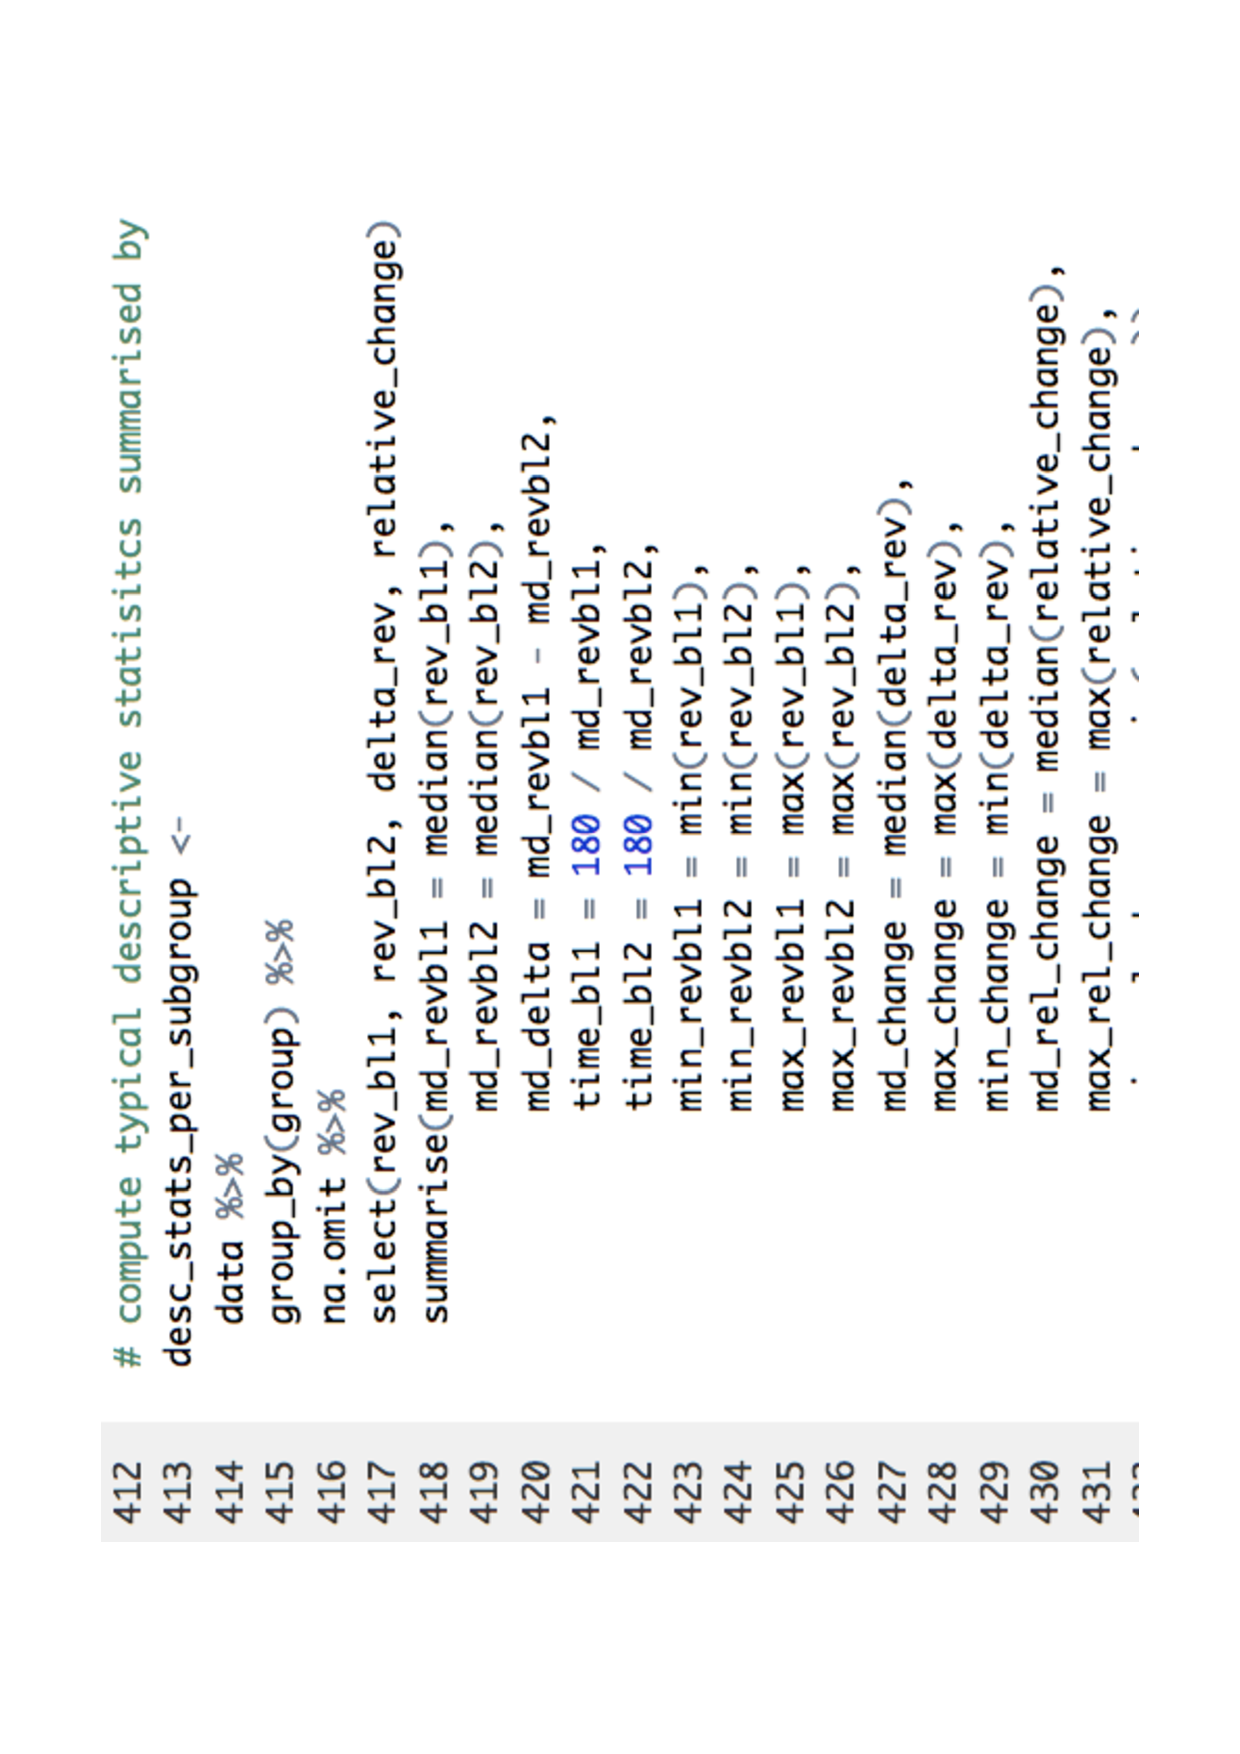
\includegraphics[valign=T,scale=.4, angle=270]{logo/rcode_example}
             \caption{$\sim$ 1000 lines of code in your paper} 
          \end{figure}
          \end{minipage}
          \begin{minipage}[t]{0.55\textwidth}
          \begin{figure}[ht]
             \centering
             
\includegraphics[valign=T,scale=.5]{logo/paper_icon}
                 \caption{ $\sim$ 20 numbers as results of computations somewhere in your paper} 
           \end{figure}
          \end{minipage}   
          \newline
          Assume there is not a direct link of your (statistical) computations to the respective number in the text.
          It will be hard to understand for someone unfamiliar with your work which calculations have yielded some figure in your paper. So confirming that the calculations are valid will be hard.  
         \end{block}     

      
      
  \begin{block}{Software tools for reproducible writing}
    
\begin{tabulary}{1.0\textwidth}{CLL}
  \hline
 Logo  & Name & Description  \\ 
 \hline

\includegraphics[valign=T,scale=.2]{logo/R_logo} & \textbf{R }& Environment for statistical calculations and programming \cite{RCoreTeam2015}\\
 
\includegraphics[valign=T,scale=.08]{logo/RStudio_logo} &  \textbf{R-Studio} & IDE for R including features for version control (eg git), and literal programming (Knitr, Pandoc, Markdown)\\
 
\includegraphics[valign=T, scale=.5]{logo/knitr_logo} &  \textbf{Knitr} & R-package to ``knit'' (or ``weave'') R-code into plain text as a way of functional programming \cite{Xie2016}\\
 
\includegraphics[valign=T, scale=.3]{logo/git_logo} & \textbf{Git} & version control tool, handles multiples collaborators, tracks changes in text files\\
 \texttt{PANDOC} &  \textbf{Pandoc} & ``swiss army knife'' for converting markup text, eg. Markdown $\rightarrow$ PDF\\
 
\includegraphics[valign=T, scale=.5]{logo/markdown_logo} & \textbf{Markdown} & Similar aims as Latex, but you learn it in 5 minutes.\\  
 %\hline
  \end{tabulary}
  
   \end{block}



        \begin{block}{Main commands to turn R+Markup-Text into polished PDF-paper}
        
       
          \begin{itemize}
             \item Weave code in text using \textbf{knitr}, giving a R-Markdown (.rmd) (or R-Latex, .rnw) file: ``Mean reaction time was \texttt{`round(mean(rt), 2)'} ms''. $\rightarrow$ ``Mean reaction time was 433.30 ms''.
             \item Knit R-Text-Mixup to pure text plus markup using R-package \textbf{knitr:}
             \newline \texttt{knitr(source.rmd)} 
             \item Convert Markdown to Latex-PDF with \textbf{Pandoc:} 
             \newline \texttt{pandoc source.md --output paper.pdf ...} 
      \end{itemize}
          
        \end{block}
        
        
        
        \begin{block}{Conclusion}
            \begin{itemize}
            \item Note that complex cognitive steps such as creative thinking, drafting a paper outline, writing an argument, debugging code etc. are best dealt with sequentially, as depicted in the workflow. Our brain is not so fit for multitasking \cite{Clapp2011}.
             \item A great combination of tools for efficient and reproducible writing papers is: R+RStudio+knitr+markdown+pandoc+git.    
             \item Writing in \texttt{Markdown} is nice, because little markup clutters the view. Pandoc then compiles to latex, applying some Tex-template of your flavor.
             \item However,  \texttt{Pandoc} is not (yet) flexible enough to adjust every layout detail one may think of. 
             \item Slides using \texttt{Markdown} or {Latex/Beamer} are no pleasure to the eay.
             \item Looking forward to the time when it is possible to write in R+Markdown and compile to Tex easily with all kinds of style-templates!
                \end{itemize}
        \end{block}     



     \begin{block}{References}
     \begin{tiny}
   
     %https://github.com/sebastiansauer/Poster_repro_paper_writing \\
     \bibliographystyle{plain}
     \bibliography{bibliography}
     \end{tiny}
     \end{block}     
   
   
         \end{column}
    \end{columns}
  \end{frame}
\end{document}


%%%%%%%%%%%%%%%%%%%%%%%%%%%%%%%%%%%%%%%%%%%%%%%%%%%%%%%%%%%%%%%%%%%%%%%%%%%%%%%%%%%%%%%%%%%%%%%%%%%%
%%% Local Variables: 
%%% mode: latex
%%% TeX-PDF-mode: t
%%% End:
